\section{IllustrisTNGのデータの取り扱い}
%Illustris-TNGは、銀河形成をシミュレーションする大規模な磁気流体力学シミュレーションのシリーズで、2017年に発表されたIllustrisプロジェクトの後継として、より高解像度とより正確な物理モデルを備えている。
%
%Illustris-TNGは、暗黒物質、ガス、星の3つの物質成分をシミュレートします。暗黒物質は、銀河の重力を支配する仮説上の粒子で、ガスは銀河の星形成の材料となり、星は銀河の光源となります。
%
%Illustris-TNGは、銀河の形成と進化のさまざまな側面をシミュレートします。具体的には、以下のようなことをシミュレートします。
%
%* 銀河の形成と進化
%* 銀河の構造と組成
%* 銀河の相互作用
%* 銀河の進化の歴史
%
%Illustris-TNGは、銀河形成の理解を深めるために重要なツールです。シミュレーション結果は、銀河の観測結果と比較することで、銀河形成の物理モデルを検証し、改善するために使用できます。
%
%Illustris-TNGは、3つの異なる解像度で実行されています。
%
%* TNG50:50億パーセク(約160億光年)の体積を、約5000万個の粒子でシミュレートします。
%* TNG100:100億パーセク(約320億光年)の体積を、約10億個の粒子でシミュレートします。
%* TNG300:300億パーセク(約960億光年)の体積を、約100億個の粒子でシミュレートします。
%
%Illustris-TNGのデータは、一般に公開されています。このデータは、銀河形成の研究を行う研究者や学生が使用できます。

Illustris-TNGはVolker Springelが率いて作られた最先端の宇宙論的銀河形成シミュレーションで,銀河形成を促進する様々な物理過程を考慮しながら,ビッグバン直後から現在までの模擬宇宙の広い範囲をシミュレーションしている.シミュレーションデータはTNG50,TNG100,TNG300の3つが存在し,それぞれ空間体積が\SI{50}{Mpc},\SI{100}{Mpc},\SI{300}{Mpc}の立法体内でシミュレーションを行っている.最も大きいTNG300は,銀河団などの珍しい天体の解析が可能であり,最大の銀河サンプルが得られる.一方,体積の小さいTNG50では,希少天体のサンプリングは比較的限定されるが,TNG300に比べ質量分解能は数百倍高く,銀河の構造的性質,銀河周辺のガスの詳細な構造,物理モデルの収束性などをより詳細に調べることができる.そこで本研究ではTNG50-1を利用して解析を行う.

%\begin{table}[htbp]
%	\centering
%	\caption{}
%	\label{tab:}
%	\begin{tabular}{ccccc}
%		\toprule
%		&  & TNG50 & TNG100 & TNG300 \\
%		\midrule
%		Volume & [\si{Mpc^3}] & $51.7^3$ & $110.7^3$ & $302.6^3$ \\
%		$L_\text{box}$& [\si{Mpc}/h] & 35 & 75  & 205 \\
%		$N_\text{GAS}$& - & $2160^3$ & $1820^3$ & $2500^3$ \\
%		$N_\text{DM}$& - & $2160^3$ & $1820^3$ & $2500^3$ \\
%		$N_\text{TR}$& - & $2160^3$ & $2\times1820^3$ & $2500^3$ \\
%		$m_\text{baryon}$& [\si{M_\odot}] & \num{8.5e+4} & \num{1.4e+4} & \num{1.1e+7} \\
%		$m_\text{DM}$& [\si{M_\odot}] & \num{4.5e+4} & \num{7.5e+4} & \num{5.9e+7} \\
%		$\epsilon_\text{gas,min}$ & [pc] & 74 & 185 & 370 \\
%		$\epsilon_\text{DM,*}$ & [pc] & 288 & 740 & 1480 \\
%		\bottomrule
%	\end{tabular}
%\end{table}
%
%\clearpage

Illustrisプロジェクトのシミュレーションを含め,Illustris-TNGプロジェクトのシミュレーションデータは以下の通りが公開されている.

\begin{figure}[H]
	\centering
	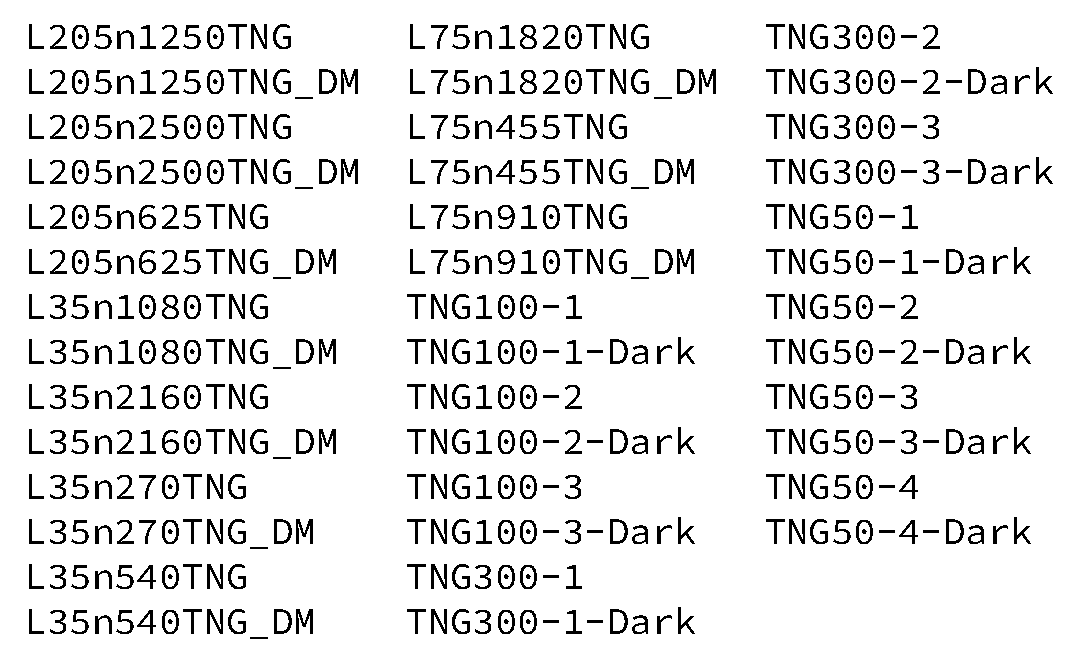
\includegraphics[width=0.7\linewidth]{./pic/ALLsimTNG.pdf}
\end{figure}

シミュレーションデータのディレクトリ下には次のようなディレクトリとファイルが存在する:\texttt{output/},\texttt{processing/},\texttt{simulation.hdf5}

\texttt{output/}ディレクトリ下には,グループカタログ,スナップショット,Subboxなどのデータが存在する.グループカタログにはHalo(銀河団)カタログやSubhalo(銀河)カタログが存在する.スナップショットには宇宙誕生を0として,現在を99として100個のスナップショットファイルが存在する.例えばTNG50-1の場合,宇宙誕生から0.179 Gyrをスナップショット0として13.803 Gyrをスナップショット99としている.ディレクトリ「\texttt{groups\_*}」,「\texttt{snapdir\_*}」の\texttt{*}には3桁でスナップショット番号が入る.現在の宇宙(スナップショット99)を使用したい場合は,ディレクトリ「\texttt{groups\_099}」,「\texttt{snapdir\_099}」を見れば良い.

そのディレクトリ下には,グループカタログやスナップショットのデータは大きいため,複数のファイルに分割されていて,これをチャンクファイルという. グループカタログのチャンクファイルは「\texttt{fof\_subhalo\_tab\_*}」もしくは「\texttt{groups\_*}」のファイル名でで定義され連番表記されている.


各スナップショットには、FoFとSubfindオブジェクトの両方を含むグループカタログが1つずつ関連付けられています。グループファイルは、生のスナップショットと同様に、少数のサブファイルに分割されます。TNGでは、これらのファイルは "fof\_subhalo\_tab\_*"と呼ばれていますが、オリジナルのIllustrisでは "groups\_*"と呼ばれていました(それ以外は基本的に同じです)。すべてのHDF5グループカタログは次のグループを含む: Header, Group, Subhalo. 各グループ/サブグループのメンバー粒子のIDは、グループカタログファイルには格納されていません。むしろ、スナップショットファイル内の粒子/セルは、グループメンバーシップに従って並べられます。

混乱を避けるため、異なるタイプのオブジェクトを指す場合は以下の用語を使用します:

    "Group"、"FoF Group"、"FoF Halo "はすべてハローを指す。
    「サブグループ","サブハロ","サブファインドグループ "は全てサブハロを指す。
    各ハローの最初の(最も質量の大きい)サブグループは、"プライマリー・サブグループ "または "セントラル・サブグループ "です。
    同じハロー内の他のサブグループはすべて「セカンダリーサブグループ」または「サテライトサブグループ」です。
